\chapter{$\mathbf{n\equiv 7,8\textbf{(mod 14)}}$} \label{chap:7,8 (mod 14)}
In this chapter, we will use our own constructions based on edge lengths in $K_{n}$ where $n \equiv 7\text{ or }8 \pmod{14}$. We begin by describing our construction and then later formallize these ideas in the results section.
\section{Construction}\label{sec:7,8constr}
The minimum number of vertices in a forest on seven edges is $9$ (like in $\mathbf{T_{7}^{11}\sqcup T_{2}^{1}}$) but $K_{7}$ and $K_{8}$ each have less vertices than that, so none of our forests could be a subgraph of either one. For this reason, $K_{21}$ and $K_{22}$ are the base graphs for decomposing $K_{n}$ where $n\equiv 7\text{ and }8$, respectively, into seven edge forests.
\begin{figure}[H]
    \begin{center}
      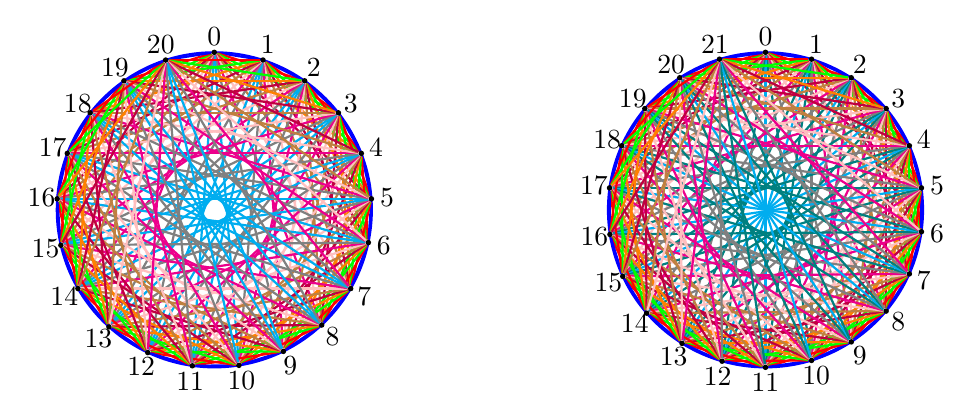
\begin{tikzpicture}[scale=2,
        dot/.style={circle, fill=black, minimum size=2pt, inner sep=0pt},
        lbl/.style={draw=none, fill=none, inner sep=0pt, anchor=center}
      ]
  
          \draw[blue, thick] (0,0) circle (1);
          \foreach \i in {0,...,20} {
            \pgfmathtruncatemacro{\angle}{90 - \i*360/21}
            \node[dot] (a\i) at (\angle:1) {};
            \node[lbl] at (\angle:1.1) {\i};
          }
          \foreach \i in {0,...,20} {
            \foreach \j in {0,...,20} {
              \ifnum\j>\i\relax
                \pgfmathtruncatemacro{\d}{mod(\j-\i,21)}
                \pgfmathtruncatemacro{\dmin}{min(\d,21-\d)}
                \ifnum\dmin=1   \draw[blue,   thick] (a\i) -- (a\j); \fi
                \ifnum\dmin=2   \draw[red,    thick] (a\i) -- (a\j); \fi
                \ifnum\dmin=3   \draw[green,  thick] (a\i) -- (a\j); \fi
                \ifnum\dmin=4   \draw[orange, thick] (a\i) -- (a\j); \fi
                \ifnum\dmin=5   \draw[purple, thick] (a\i) -- (a\j); \fi
                \ifnum\dmin=6   \draw[brown,  thick] (a\i) -- (a\j); \fi
                \ifnum\dmin=7   \draw[pink,   thick] (a\i) -- (a\j); \fi
                \ifnum\dmin=8   \draw[magenta,thick] (a\i) -- (a\j); \fi
                \ifnum\dmin=9   \draw[gray,   thick] (a\i) -- (a\j); \fi
                \ifnum\dmin=10  \draw[cyan,   thick] (a\i) -- (a\j); \fi
              \fi
            }
          }
  
        % K_22
        \begin{scope}[shift={(3.5,0)}]
          \draw[blue, thick] (0,0) circle (1);
          \foreach \i in {0,...,21} {
            \pgfmathtruncatemacro{\angle}{90 - \i*360/22}
            \node[dot] (b\i) at (\angle:1) {};
            \node[lbl] at (\angle:1.1) {\i};
          }
          \foreach \i in {0,...,21} {
            \foreach \j in {0,...,21} {
              \ifnum\j>\i\relax
                \pgfmathtruncatemacro{\d}{mod(\j-\i,22)}
                \pgfmathtruncatemacro{\dmin}{min(\d,22-\d)}
                \ifnum\dmin=1   \draw[blue,   thick] (b\i) -- (b\j); \fi
                \ifnum\dmin=2   \draw[red,    thick] (b\i) -- (b\j); \fi
                \ifnum\dmin=3   \draw[green,  thick] (b\i) -- (b\j); \fi
                \ifnum\dmin=4   \draw[orange, thick] (b\i) -- (b\j); \fi
                \ifnum\dmin=5   \draw[purple, thick] (b\i) -- (b\j); \fi
                \ifnum\dmin=6   \draw[brown,  thick] (b\i) -- (b\j); \fi
                \ifnum\dmin=7   \draw[pink,   thick] (b\i) -- (b\j); \fi
                \ifnum\dmin=8   \draw[magenta,thick] (b\i) -- (b\j); \fi
                \ifnum\dmin=9   \draw[gray,   thick] (b\i) -- (b\j); \fi
                \ifnum\dmin=10  \draw[teal,   thick] (b\i) -- (b\j); \fi
                \ifnum\dmin=11  \draw[cyan,   thick] (b\i) -- (b\j); \fi
              \fi
            }
          }
        \end{scope}
  
      \end{tikzpicture}
    \end{center}
    \caption{$K_{21}$ (left) and $K_{22}$ (right) with edges colored by length.}
    \label{fig:K21K22colored}
  \end{figure}
  Here is problem with this case relative to our forests on seven edges. $K_{21}$ has lengths \textcolor{blue}{1} through \textcolor{cyan}{10} and $K_{21}$ has lengths \textcolor{blue}{1} through \textcolor{cyan}{11}. So the number of distinct lengths in the base graphs is no longer $7$. Furthermore, $K_{22}$ has one more length than $K_{21}$. This means we cannot just fit $7$ distinct lengths on a single labeling and collect all edges when we develop the vertices by $1$. However, new lengths still come $7$ at a time at each step $t\mapsto t+1$: $K_{14t+7}$ and $K_{14t+8}$ have lengths in $\{1,\hdots 10\}\cup \cdots\cup\{7t-3,\hdots,3+7t\}$ and $\{1,\hdots 11\}\cup \cdots\cup\{7t-2,\hdots,4+7t\}$, respectively.

  If we could just take care of lengths $\{1,2,3\}$ and $\{1,2,3,\infty \}$, respectively, we could just use some rosa-type labeling to collect each of the remaining lengths using some rosa-type labeling, since $7$ lengths will remain. Before we think about that, recall that in $K_{22}$ there will only be $11$ edges of length $11$. We want to make sure we are wary of that as well. We want the number of each length to be the same to generate them with a labeling.

 So, we redefine length of edges and development for vertices in $K_{22}$:
$$\ell(uv)=\begin{cases}\min\{|u-v|,21-|u-v|\}, & u,v\neq \infty, \\ \infty, & u\text{ or }v=\infty \end{cases} \text{ and }v\mapsto 
\begin{cases}
  v+1,&v\in\mathbb{Z}_{n-1},\\
  \infty,        &v=\infty.
  \end{cases}$$
  If we do this, we will have $21$ edges of lengths $1$ through $6$ as well as $\infty$, since the infinity node will have all $21$ edges of length $\infty$ to nodes in $\ZZ_{21}$ incident to it. So if we partition the edges by these notions of length, we can now cyclically generate all edges of $K_{21}$ and $K_{22}$ with labelings. Now the only problem is that there are still $10$ and $11$ distinct lengths in $K_{21}$ and $K_{21}$, respectively.

  \begin{figure}[H]
    \begin{center}
      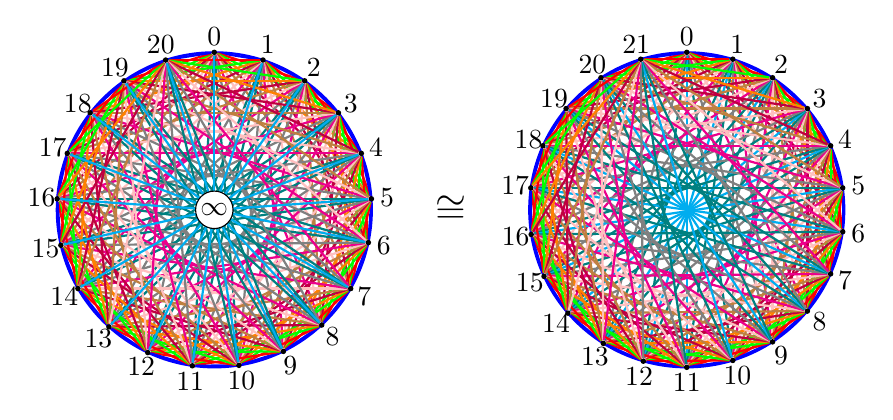
\begin{tikzpicture}[scale=2]
        \tikzset{
          dot/.style={circle, fill=black, minimum size=2pt, inner sep=0pt},
          lbl/.style={draw=none, fill=none, inner sep=0pt, anchor=center}
        }
  
        % — Left: K_{21} ∪ {∞} —
        \begin{scope}
          % outer circle for reference
          \draw[blue, thick] (0,0) circle (1);
  
          % Z_{21} nodes
          \foreach \i in {0,...,20} {
            \pgfmathtruncatemacro{\angle}{90 - \i*360/21}
            \node[dot] (a\i) at (\angle:1) {};
            \node[lbl] at (\angle:1.1) {\i};
          }
  
          % define infinity
          \coordinate (inf) at (0,0);
  
          % edges among Z_{21}
          \foreach \i in {0,...,20} {
            \foreach \j in {0,...,20} {
              \ifnum\j>\i\relax
                \pgfmathtruncatemacro{\d}{mod(\j-\i,21)}
                \pgfmathtruncatemacro{\dmin}{min(\d,21-\d)}
                \ifnum\dmin=1   \draw[blue,   thick] (a\i) -- (a\j); \fi
                \ifnum\dmin=2   \draw[red,    thick] (a\i) -- (a\j); \fi
                \ifnum\dmin=3   \draw[green,  thick] (a\i) -- (a\j); \fi
                \ifnum\dmin=4   \draw[orange, thick] (a\i) -- (a\j); \fi
                \ifnum\dmin=5   \draw[purple, thick] (a\i) -- (a\j); \fi
                \ifnum\dmin=6   \draw[brown,  thick] (a\i) -- (a\j); \fi
                \ifnum\dmin=7   \draw[pink,   thick] (a\i) -- (a\j); \fi
                \ifnum\dmin=8   \draw[magenta,thick] (a\i) -- (a\j); \fi
                \ifnum\dmin=9   \draw[gray,   thick] (a\i) -- (a\j); \fi
                \ifnum\dmin=10  \draw[teal,   thick] (a\i) -- (a\j); \fi
              \fi
            }
          }
  
          % ∞-edges in cyan
          \foreach \i in {0,...,20} {
            \draw[cyan, thick] (inf) -- (a\i);
          }
  
          % infinity label on white background
          \node[circle, fill=white, draw=black, inner sep=1pt] at (inf) {$\infty$};
        \end{scope}
  
        % isomorphism arrow
        \node at (1.5,0) {$\Large\cong$};
  
        % — Right: K_{22} —
        \begin{scope}[shift={(3,0)}]
          % outer circle
          \draw[blue, thick] (0,0) circle (1);
  
          % Z_{22} nodes
          \foreach \i in {0,...,21} {
            \pgfmathtruncatemacro{\angle}{90 - \i*360/22}
            \node[dot] (b\i) at (\angle:1) {};
            \node[lbl] at (\angle:1.1) {\i};
          }
  
          % edges colored by minimal distance
          \foreach \i in {0,...,21} {
            \foreach \j in {0,...,21} {
              \ifnum\j>\i\relax
                \pgfmathtruncatemacro{\d}{mod(\j-\i,22)}
                \pgfmathtruncatemacro{\dmin}{min(\d,22-\d)}
                \ifnum\dmin=1   \draw[blue,   thick] (b\i) -- (b\j); \fi
                \ifnum\dmin=2   \draw[red,    thick] (b\i) -- (b\j); \fi
                \ifnum\dmin=3   \draw[green,  thick] (b\i) -- (b\j); \fi
                \ifnum\dmin=4   \draw[orange, thick] (b\i) -- (b\j); \fi
                \ifnum\dmin=5   \draw[purple, thick] (b\i) -- (b\j); \fi
                \ifnum\dmin=6   \draw[brown,  thick] (b\i) -- (b\j); \fi
                \ifnum\dmin=7   \draw[pink,   thick] (b\i) -- (b\j); \fi
                \ifnum\dmin=8   \draw[magenta,thick] (b\i) -- (b\j); \fi
                \ifnum\dmin=9   \draw[gray,   thick] (b\i) -- (b\j); \fi
                \ifnum\dmin=10  \draw[teal,   thick] (b\i) -- (b\j); \fi
                \ifnum\dmin=11  \draw[cyan,   thick] (b\i) -- (b\j); \fi
              \fi
            }
          }
        \end{scope}
  
      \end{tikzpicture}
    \end{center}
    \caption{$K_{21}\vee K_{1}$ is isomorphic to $K_{22}$ (right)}
    \label{fig:K21K22infty}
  \end{figure}

  Now, let's begin by looking at $K_{21}$. How can we collect $21$ edges of length $1,2,\text{ and }3$? Well, what if we have some labelings that generate $21$ distinct edges of length $8,9\text{ and }10$ between them? What if we can do something similar for $K_{22}$ with edges of lengths $1,2,3,\text{ and }\infty$? By imposing a new edge label on top of the standard length $\ell$, we can can achieve this. We define $\ell_{7}^{+}$ from $\ZZ_{21}\cup\{\infty\}\text{ to }\ZZ_{7}$ as follows
  $$\ell_{7}^{+}(uv)=\begin{cases} u+v\textbf{ mod }14, & u,v\neq \infty\\ v, &u=\infty \end{cases}$$
  Now, every edge has a standard length $\ell$ and an additive length $\ell_{7}^{+}$ modulo $7$. Previously, we partitioned the edges into sets $E_{i}$ of edges of length $i$ for each length $i\in \{1,\hdots, 10\}$ via the standard length function $\ell$. Now, within each set $E_{i}$ of length $i$, we have further partitioned the edges into sets $E_{i,j}$ of standard length $i$ and additive length $j$ modulo $7$. For example: the edge $(1,8)$ has length $\ell((1,8))=7$ and $\ell_{7}^{+}((1,8))=8+1 \textbf{ mod }7=2$, so $(1,8)\in E_{7,2}$. Here is a labeling of $\mathbf{T_{6}^{6}}\sqcup \mathbf{T_{3}^{1}}$ that utilizes this new partition.

  \begin{figure}[H]
    \begin{center}
      
      \begin{tikzpicture}[scale=1]
        %-----------------------------------------column 1----------------------------------------------------------------
        \tikzset{
            dot/.style={circle, fill=black, minimum size=4pt, inner sep=0pt},
            lbl/.style={draw=none, fill=none, inner sep=0pt, anchor=center}
          }
        % — Labeling 1 —
        \begin{scope}
          \matrix (arr1) [draw,
                          anchor=east,
                          matrix of nodes,
                          nodes={minimum size=0.5cm, inner sep=0pt, anchor=center}
                         ] at (-1.5,0) {
            $\textcolor{blue}{1}_{3}$ & $\textcolor{blue}{1}_{5}$ & $\textcolor{blue}{1}_{2}$ \\
            $\textcolor{red}{2}_{2}$  & $\textcolor{red}{2}_{6}$  & $\textcolor{green}{3}_{0}$ \\
                                      & $\textcolor{green}{3}_{4}$ &                      \\
          };
  
          \node[dot,label=above left:2] (C1)  at (0,0)    {};
          \node[dot,label=above:0]      (L10) at (90:0.5)  {};
          \node[dot,label=left:1]       (L11) at (162:0.5){};
          \node[dot,label=left:3]       (L13) at (234:0.5){};
          \node[dot,label=right:4]      (L14) at (306:0.5){};
          \node[dot,label=right:5]      (L15) at (18:0.5) {};
  
          \draw[red,   thick]   (C1) -- (L10);
          \draw[blue,  thick]   (C1) -- (L11);
          \draw[blue,  thick]   (C1) -- (L13);
          \draw[red,   thick]   (C1) -- (L14);
          \draw[green, thick]   (C1) -- (L15);
  
          \node[dot,label=below:12] (P12) at (-0.5,-1) {};
          \node[dot,label=below:11] (P11) at ( 0  ,-1) {};
          \node[dot,label=below:14] (P14) at ( 0.5,-1) {};
  
          \draw[blue,  thick] (P12) -- (P11);
          \draw[green, thick] (P11) -- (P14);

          \node at (1.5,0) {\scriptsize $\overset{+7}{\longrightarrow}$};

        \end{scope}
  
        % — Labeling 2 —
        \begin{scope}[yshift=-3cm]
          \matrix (arr2) [draw,
                          anchor=east,
                          matrix of nodes,
                          nodes={minimum size=0.5cm, inner sep=0pt, anchor=center}
                         ] at (-1.5,0) {
            $\textcolor{blue}{1}_{4}$ & $\textcolor{blue}{1}_{6}$ & $\textcolor{red}{2}_{3}$ \\
            $\textcolor{red}{2}_{0}$  & $\textcolor{red}{2}_{5}$  & $\textcolor{green}{3}_{1}$ \\
                                      & $\textcolor{green}{3}_{6}$ &                      \\
          };
  
          \node[dot,label=above left:6] (C2)  at (0,0)    {};
          \node[dot,label=above:4]      (L24) at (90:0.5)  {};
          \node[dot,label=left:5]       (L25) at (162:0.5){};
          \node[dot,label=left:7]       (L27) at (234:0.5){};
          \node[dot,label=right:8]      (L28) at (306:0.5){};
          \node[dot,label=right:9]      (L29) at (18:0.5) {};
  
          \draw[red,   thick]   (C2) -- (L24);
          \draw[blue,  thick]   (C2) -- (L25);
          \draw[blue,  thick]   (C2) -- (L27);
          \draw[red,   thick]   (C2) -- (L28);
          \draw[green, thick]   (C2) -- (L29);
  
          \node[dot,label=below:14] (P214) at (-0.5,-1) {};
          \node[dot,label=below:12] (P212) at ( 0  ,-1) {};
          \node[dot,label=below:15] (P215) at ( 0.5,-1) {};
  
          \draw[red,   thick]   (P214) -- (P212);
          \draw[green, thick]   (P212) -- (P215);
          \node at (1.5,0) {\scriptsize $\overset{+7}{\longrightarrow}$};
        \end{scope}
  
        % — Labeling 3 —
        \begin{scope}[yshift=-6cm]
          \matrix (arr3) [draw,
                          anchor=east,
                          matrix of nodes,
                          nodes={minimum size=0.5cm, inner sep=0pt, anchor=center}
                         ] at (-1.5,0) {
            $\textcolor{blue}{1}_{0}$ & $\textcolor{blue}{1}_{1}$ & $\textcolor{red}{2}_{4}$ \\
            $\textcolor{red}{2}_{1}$  & $\textcolor{green}{3}_{3}$ & $\textcolor{green}{3}_{2}$ \\
                                      & $\textcolor{green}{3}_{5}$ &                      \\
          };
  
          \node[dot,label=above left:3] (C3)  at (0,0)    {};
          \node[dot,label=above:0]      (L30) at (90:0.5)  {};
          \node[dot,label=left:1]       (L31) at (162:0.5){};
          \node[dot,label=left:4]       (L34) at (234:0.5){};
          \node[dot,label=right:5]      (L35) at (306:0.5){};
          \node[dot,label=right:6]      (L36) at (18:0.5) {};
  
          \draw[green, thick]   (C3) -- (L30);
          \draw[red,   thick]   (C3) -- (L31);
          \draw[blue,  thick]   (C3) -- (L34);
          \draw[red,   thick]   (C3) -- (L35);
          \draw[green, thick]   (C3) -- (L36);
  
          \node[dot,label=below:11] (P311) at (-0.5,-1) {};
          \node[dot,label=below:8]  (P38)  at ( 0  ,-1) {};
          \node[dot,label=below:7]  (P37)  at ( 0.5,-1) {};
  
          \draw[green, thick] (P311) -- (P38);
          \draw[blue,  thick] (P38)  -- (P37);
          \node at (1.5,0) {\scriptsize $\overset{+7}{\longrightarrow}$};
        \end{scope}

        %-------------------------------------------column2-----------------------------------------------------------------
        % — Labeling 1 —
        \begin{scope}[shift={(3,0)}]
            \node[dot,label=above left:9] (C1)  at (0,0)    {};
          \node[dot,label=above:7]      (L10) at (90:0.5)  {};
          \node[dot,label=left:8]       (L11) at (162:0.5){};
          \node[dot,label=left:10]       (L13) at (234:0.5){};
          \node[dot,label=right:11]      (L14) at (306:0.5){};
          \node[dot,label=right:12]      (L15) at (18:0.5) {};
  
          \draw[red,   thick]   (C1) -- (L10);
          \draw[blue,  thick]   (C1) -- (L11);
          \draw[blue,  thick]   (C1) -- (L13);
          \draw[red,   thick]   (C1) -- (L14);
          \draw[green, thick]   (C1) -- (L15);
  
          \node[dot,label=below:19] (P12) at (-0.5,-1) {};
          \node[dot,label=below:18] (P11) at ( 0  ,-1) {};
          \node[dot,label=below:0] (P14) at ( 0.5,-1) {};
  
          \draw[blue,  thick] (P12) -- (P11);
          \draw[green, thick] (P11) -- (P14);
          \node at (1.5,0) {\scriptsize $\overset{+7}{\longrightarrow}$};
        \end{scope}

        % — Labeling 2 —
        \begin{scope}[shift={(3,-3)}]
            \node[dot,label=above left:13] (C2)  at (0,0)    {};
            \node[dot,label=above:11]      (L24) at (90:0.5)  {};
            \node[dot,label=left:12]       (L25) at (162:0.5){};
            \node[dot,label=left:14]       (L27) at (234:0.5){};
            \node[dot,label=right:15]      (L28) at (306:0.5){};
            \node[dot,label=right:16]      (L29) at (18:0.5) {};
    
            \draw[red,   thick]   (C2) -- (L24);
            \draw[blue,  thick]   (C2) -- (L25);
            \draw[blue,  thick]   (C2) -- (L27);
            \draw[red,   thick]   (C2) -- (L28);
            \draw[green, thick]   (C2) -- (L29);
    
            \node[dot,label=below:0] (P214) at (-0.5,-1) {};
            \node[dot,label=below:19] (P212) at ( 0  ,-1) {};
            \node[dot,label=below:1] (P215) at ( 0.5,-1) {};
    
            \draw[red,   thick]   (P214) -- (P212);
            \draw[green, thick]   (P212) -- (P215);
            \node at (1.5,0) {\scriptsize $\overset{+7}{\longrightarrow}$};
            \end{scope}

            % — Labeling 3 —
            \begin{scope}[shift={(3,-6)}]
                \node[dot,label=above left:10] (C3)  at (0,0)    {};
                \node[dot,label=above:7]      (L30) at (90:0.5)  {};
                \node[dot,label=left:8]       (L31) at (162:0.5){};
                \node[dot,label=left:11]       (L34) at (234:0.5){};
                \node[dot,label=right:12]      (L35) at (306:0.5){};
                \node[dot,label=right:13]      (L36) at (18:0.5) {};
        
                \draw[green, thick]   (C3) -- (L30);
                \draw[red,   thick]   (C3) -- (L31);
                \draw[blue,  thick]   (C3) -- (L34);
                \draw[red,   thick]   (C3) -- (L35);
                \draw[green, thick]   (C3) -- (L36);
        
                \node[dot,label=below:18] (P311) at (-0.5,-1) {};
                \node[dot,label=below:16]  (P38)  at ( 0  ,-1) {};
                \node[dot,label=below:14]  (P37)  at ( 0.5,-1) {};
        
                \draw[green, thick] (P311) -- (P38);
                \draw[blue,  thick] (P38)  -- (P37);
                \node at (1.5,0) {\scriptsize $\overset{+7}{\longrightarrow}$};
                \end{scope}

        %-------------------------------------------column2-----------------------------------------------------------------
            % — Labeling 1 —
            \begin{scope}[shift={(6,0)}]
                \node[dot,label=above left:16] (C1)  at (0,0)    {};
                \node[dot,label=above:14]      (L10) at (90:0.5)  {};
                \node[dot,label=left:15]       (L11) at (162:0.5){};
                \node[dot,label=left:17]       (L13) at (234:0.5){};
                \node[dot,label=right:18]      (L14) at (306:0.5){};
                \node[dot,label=right:19]      (L15) at (18:0.5) {};

                \draw[red,   thick]   (C1) -- (L10);
                \draw[blue,  thick]   (C1) -- (L11);
                \draw[blue,  thick]   (C1) -- (L13);
                \draw[red,   thick]   (C1) -- (L14);
                \draw[green, thick]   (C1) -- (L15);

                \node[dot,label=below:5] (P12) at (-0.5,-1) {};
                \node[dot,label=below:4] (P11) at ( 0  ,-1) {};
                \node[dot,label=below:7] (P14) at ( 0.5,-1) {};

                \draw[blue,  thick] (P12) -- (P11);
                \draw[green, thick] (P11) -- (P14);
            \end{scope}

            % — Labeling 2 —
            \begin{scope}[shift={(6,-3)}]
                \node[dot,label=above left:20] (C2)  at (0,0)    {};
                \node[dot,label=above:18]      (L24) at (90:0.5)  {};
                \node[dot,label=left:19]       (L25) at (162:0.5){};
                \node[dot,label=left:0]       (L27) at (234:0.5){};
                \node[dot,label=right:1]      (L28) at (306:0.5){};
                \node[dot,label=right:2]      (L29) at (18:0.5) {};

                \draw[red,   thick]   (C2) -- (L24);
                \draw[blue,  thick]   (C2) -- (L25);
                \draw[blue,  thick]   (C2) -- (L27);
                \draw[red,   thick]   (C2) -- (L28);
                \draw[green, thick]   (C2) -- (L29);

                \node[dot,label=below:7] (P214) at (-0.5,-1) {};
                \node[dot,label=below:5] (P212) at ( 0  ,-1) {};
                \node[dot,label=below:8] (P215) at ( 0.5,-1) {};

                \draw[red,   thick]   (P214) -- (P212);
                \draw[green, thick]   (P212) -- (P215);
                \end{scope}

                % — Labeling 3 —
                \begin{scope}[shift={(6,-6)}]
                    \node[dot,label=above left:17] (C3)  at (0,0)    {};
                    \node[dot,label=above:14]      (L30) at (90:0.5)  {};
                    \node[dot,label=left:15]       (L31) at (162:0.5){};
                    \node[dot,label=left:18]       (L34) at (234:0.5){};
                    \node[dot,label=right:19]      (L35) at (306:0.5){};
                    \node[dot,label=right:20]      (L36) at (18:0.5) {};
            
                    \draw[green, thick]   (C3) -- (L30);
                    \draw[red,   thick]   (C3) -- (L31);
                    \draw[blue,  thick]   (C3) -- (L34);
                    \draw[red,   thick]   (C3) -- (L35);
                    \draw[green, thick]   (C3) -- (L36);
            
                    \node[dot,label=below:4] (P311) at (-0.5,-1) {};
                    \node[dot,label=below:2]  (P38)  at ( 0  ,-1) {};
                    \node[dot,label=below:0]  (P37)  at ( 0.5,-1) {};
            
                    \draw[green, thick] (P311) -- (P38);
                    \draw[blue,  thick] (P38)  -- (P37);
                    \end{scope}



      \end{tikzpicture}
    \end{center}
    \caption{Three labelings of $\mathbf{T_{6}^{6}}\sqcup \mathbf{T_{3}^{1}}$ (left column) that generate all edges of lengths $1,2,\text{ and }3$ in $K_{21}$ when developed by $7$ repeatedly.}
    \label{fig:K21labelingex}
  \end{figure}

  The squares to the left of the labelings contain the standard lengths $\ell$ with the same colors we have been using, and then the new length $\ell_{7}^{+}$ in black as the subscript, for each of the seven edges in each labeling. If you look at each edge length, you will find that there is a representative for each equivalence class via $\ell_{7}^{+}$ somewhere exactly once across the three labelings.

  Such $K_{n}$ are of the form $K_{14t+7}$ and $K_{14t+8}$ where $t\geq 1$. $K_{7}$ and $K_{8}$ only have $7$ and $8$ distinct vertices, respectively, and since the minimum number of distinct vertices a forest on seven edges (such as $\mathbf{T_{7}^{11}\sqcup T_{2}^{1}}$) has is $9$ vertices, it is impossible for any seven edge forest to even be a subgraph of $K_{7}$ and $K_{8}$. So $K_{21}$ and $K_{22}$ are the base graphs for $K_{n}$ where $n\equiv 7\text{ or }8\pmod{14}$.
\section{Results}\label{sec:7,8result}

\begin{definition}\label{def:1-2-3}
    Let $G$ be a graph with $7$ edges. A (1-2-3)-\emph{labeling} of $3G$ is an assignment $f$ of the integers $\{0,\dots,20\}$ to the vertices of $3G$ such that
    \begin{enumerate}
        \item $f(u) \neq f(v)$ whenever $u$ and $v$ belong to the same connected component,
        \item[] and
        %\item there are exactly $7$ edges of length $i$ for each $i \in \{1,2,3\}$, and
       % \item if two edges $u_1v_1$ and $u_2v_2$ are of length $i$ and $u_1 \equiv v_1 \pmod7$, then $u_2 \not \equiv v_2 \pmod7.$
      %  \item when $f$ is reduced modulo $7$, there is exactly one edge of length $j$, for $j \in \{1,2,3\}$, of the form $\{i,i+j\}$ for $i \in \{0,\dots,6\}.$
        \item $$\bigcup_{uv\in E(3G)} \{(f(u)\; \textbf{mod } 7,f(v)\; \textbf{mod } 7)\}= \bigcup_{i=0}^{6} \bigcup_{j=1}^{3} \{(i,i+j \; \textbf{mod } 7)\}.$$
    \end{enumerate}

\end{definition}
Notice that the second condition of a (1-2-3)-labeling says that $3G$ contains exactly $7$ edges of each of the lengths $1,2$, and $3$. Furthermore, no two edges of the same length have the same end labels when reduced modulo $7.$ A (1-2-3) labeling of every forest with $7$ edges with the exception of $\mathbf{T_{7}^{11}}\sqcup\mathbf{T_{2}^{1}}$ is given in Figure \ref{tab:(1-2-3)}. This exceptional forest does not admit such a labeling and is dealt with in Section \ref{chap:special case}.

\begin{thm}\label{thm:1-2-3 plus rho}
    Let $G$ be a bipartite graph with $7$ edges. If $3G$ admits a ($1$-$2$-$3$)-labeling and $G$ admits a $\rho^{+}$-labeling, then $G$ decomposes $K_{14k+7}$ for every $k\geq 1.$
\end{thm}
\begin{proof}
    Let $n=14k+7$ and notice that $K_n$ has $|E(K_n)|=(7k+3)(14k+7)$ edges, which can be partitioned into $14k+7$ edges of each of the lengths in $\{1,2,\dots,7k+3\}.$  We will construct the $G$-decomposition in two steps. First, we use the 1-2-3-labeling to identify all the edges of lengths $1,2,$ and $3$ accounting for $3(2k+1)$ copies of $G$. Then, we use the $\rho^{+}$-labeling to identify edges of the remaining lengths in $7k(2k+1)$ copies of $G$. In total, the decomposition consists of $|E(K_n)|/7=(7k+3)(2k+1)$ copies of $G.$

    % Is developing by k defined?
    Let $f_1$ be a (1-2-3)-labeling of $3G$ and identify this graph as a block $B_0$. Then develop $B_0$ by 7 modulo $n$. Since the order of the development is $\frac{n}{7}=2k+1$ and there are 7 edges of each of the lengths $1,2,$ and $3$ in $B_0$, we have identified $3(2k+1)$ copies of $G$ containing all $14k+7=n$ edges of each length $1,2,$ and $3$. Notice (2) of Definition \ref{def:1-2-3} ensures no edge has been counted more than once in the development.

    Let $f_2:V(G) \rightarrow \{0,\dots,14\}$ be a $\rho^{+}$-labeling of $G$ with associated vertex partition $(A,B).$ For $i=1,2,\dots,k,$ identify blocks $B_i \cong G$ with vertex labels $\ell$ such that
    \[
    \ell(v)=
    \begin{cases}
        f_2(v), & \textrm{if } v \in A \\
        f_2(v)+3+7(i-1), & \textrm{if } v \in B
    \end{cases}
    \]
    Notice that the $i^{\textrm{th}}$ block contains exactly one edge of each length $7i-3,7i-2, \dots,$ and $ 7i+3.$ This is because every edge $ab$ has length 
    \[
    \ell(b)-\ell(a)=f_2(b)-f_2(a)+3+7(i-1)
    \]
    and $f_2(b)-f_2(a)$ is a length in $\{1,\dots,7\}.$
    Developing each block $B_i$ by 1 yields $14k+7$ copies of $G$ per block and accounts for $14k+7$ edges of each of the lengths $4,5,\dots,$ and $7k+3$.

    Since we have identified
    \[
    3(2k+1)+k(14k+7)=(7k+3)(2k+1)
    \]
    edge-disjoint copies of $G$, the proof is complete.
    % $f_2+3, f_2 + 10, \dots, f_2 + 3+7(k-1)$
    %Because $f_2$ is a $\rho$-labeling, it induces exactly one edge of each length $1,2,\dots,7.$ Further, because it is a $\rho^{+}$-labeling, fixing the labels of the $A$ vertices and increasing the set of $B$ vertices each by an integer $c$ increases the lengths by $c.$ We call this process \emph{stretching} the edges. 
\end{proof}
%%%
To address the $n \equiv 8 \pmod{14}$ case, we define the following labeling.
\begin{definition}\label{def:1-2-3-1-rot}
    Let $G$ be a graph with $7$ edges. A \emph{1-rotational $(1$-$2$-$3)$-labeling} of $4G$ is an assignment $f$ of $\{0,\dots,20\} \cup \infty$ to the vertices of $4G$ such that
    \begin{enumerate}
        \item $f(u) \neq f(v)$ whenever $u$ and $v$ belong to the same connected component, 
        \item[] and
%\item when the integer values of $f$ are reduced modulo $7$, there is exactly one edge of length $j$, for $j \in \{1,2,3\}$, of the form $\{i,i+j\}$ for $i \in \{0,\dots,6\},$ and exactly one edge of length $\infty$ of the form $\{i,\infty\}$ for $i \in \{0,\dots,6\}.$
        \item  $$ \bigcup_{uv\in E(4G)} \{(f(u)\; \textbf{mod } 7,f(v)\; \textbf{mod } 7)\}= \bigcup_{i=0}^{6} \bigcup_{j=1}^{3} \{(i,i+j \; \textbf{mod } 7), (i,\infty)\}.$$
    \end{enumerate}
\end{definition}
Notice that the second condition of a 1-rotational (1-2-3)-labeling says that $4G$ contains exactly $7$ edges of each of the lengths $1,2,3$, and $\infty$. Furthermore, no two edges of the same length have the same end labels when reduced modulo $7.$ A 1-rotational (1-2-3)-labeling of every forest with $7$ edges with the exception of $\mathbf{T_{7}^{11}}\sqcup\mathbf{T_{2}^{1}}$ is given in Figure \ref{tab:1-rot(1-2-3)}. 

\begin{thm}\label{thm:1-2-3 1-rot plus rho}
    Let $G$ be a bipartite graph with $7$ edges. If $4G$ admits a $1$-rotational  $(1$-$2$-$3)$-labeling and $G$ admits a $\rho^{+}$-labeling, then $G$ decomposes $K_{14k+8}$ for every $k\geq1.$
\end{thm}

\begin{proof}
    Let $n=14k+8$ and notice that $K_n$ has $|E(K_n)|=(7k+4)(14k+7)$ edges, which can be partitioned into $14k+7$ edges of each of the lengths in $\{1,2,\dots,7k+3,\infty\}.$  We will construct the $G$-decomposition in two steps. First, we use the 1-rotational (1-2-3)-labeling to identify all the edges of lengths $1,2,3,$ and $\infty$ accounting for $4(2k+1)$ copies of $G$. Then, we use the $\rho^{+}$-labeling to identify edges of the remaining lengths in $7k(2k+1)$ copies of $G$. In total, the decomposition consists of $|E(K_n)|/7=(7k+4)(2k+1)$ copies of $G.$
%left off here 1/27
    Let $f_1$ be a 1-rotational (1-2-3)-labeling of $4G$ and identify this graph as a block $B_0$. Then develop $B_0$ by 7 modulo $n-1$. Since the order of the development is $\frac{n-1}{7}=2k+1$ and there are 7 edges of each of the lengths $1,2,3$ and $\infty$ in $B_0$, we have identified $4(2k+1)$ copies of $G$ containing all $14k+7=n-1$ edges of each length $1,2,3$ and $\infty$. Notice (2) of Definition \ref{def:1-2-3-1-rot} ensures no edge has been counted more than once in the development.

    Let $f_2:V(G) \rightarrow \{0,\dots,14\}$ be a $\rho^{+}$-labeling of $G$ with associated vertex partition $(A,B).$ For $i=1,2,\dots,k,$ identify blocks $B_i \cong G$ with vertex labels $\ell$ such that
    \[
    \ell(v)=
    \begin{cases}
        f_2(v), & \textrm{if } v \in A \\
        f_2(v)+3+7(i-1), & \textrm{if } v \in B
    \end{cases}
    \]
    Notice that the $i^{\textrm{th}}$ block contains exactly one edge of each length $7i-3,7i-2, \dots,$ and $ 7i+3.$ This is because every edge $ab$ has length 
    \[
    \ell(b)-\ell(a)=f_2(b)-f_2(a)+3+7(i-1)
    \]
    and $f_2(b)-f_2(a)$ is a length in $\{1,\dots,7\}.$
    Developing each block $B_i$ by 1 yields $14k+7$ copies of $G$ per block and accounts for $14k+7$ edges of each of the lengths $4,5,\dots,$ and $7k+3$.

    Since we have identified
    \[
    4(2k+1)+k(14k+7)=(7k+4)(2k+1)
    \]
    edge-disjoint copies of $G$, the proof is complete.
\end{proof}

We are now able to state the main thm of this section.
%%
\begin{thm}\label{thm:7 or 8 mod 14}
    Let $F$ be a forest with $7$ edges and $F \not \cong \mathbf{T_{7}^{11}}\sqcup\mathbf{T_{2}^{1}}$. There exists an $F$-decomposition of $K_n$ whenever $n \equiv 7 \textrm{ or } 8 \pmod{14}$ and $n \geq 21.$
\end{thm}
\begin{proof}
    If $n \equiv 7 \pmod{14},$ a (1-2-3)-labeling of $3F$ can be found in Figure \ref{tab:(1-2-3)}. On the other hand, if $n \equiv 8 \pmod{14}$, then a 1-rotational (1-2-3)-labeling of $4F$ can be found in Figure \ref{tab:1-rot(1-2-3)}. In either case, a $\rho^{+}$-labeling of $F$ can be found in Figure \ref{tab:sigmapm} (recall that a $\sigma^{+-}$-labeling is a $\rho^{+}$-labeling). The result now follows from Theorems \ref{thm:1-2-3 plus rho} and \ref{thm:1-2-3 1-rot plus rho}.
\end{proof}
%%
\begin{example}
We illustrate the constructions in the previous two theorems by finding an $F$-decomposition of $K_{35}$ and $K_{36}$ for the forest graph $F \cong \mathbf{T_{6}^{6}} \sqcup \mathbf{T_{3}^{1}}$.\newline

\noindent Here are excerpts from the preceding tables for $\mathbf{T_{6}^{6}} \sqcup \mathbf{T_{3}^{1}}$

\begin{figure}[H]
\centering
        \scalebox{0.6}{\documentclass{standalone}
\usepackage{tikz}
\usepackage{graphicx}  % For including external images
\usepackage{standalone}  % For including standalone files
\usepackage{youngtab}  % For tables
\usepackage{array}  % For \extrarowheight support
\usepackage{amsmath}
\usepackage{longtable}  % For multi-page tables

\begin{document}
\centering
\resizebox{\textwidth}{!}{%
\begin{tabular}{|c|c|}
\hline
    Labeling Type & Labelings\\
\hline
    $\sigma^{+-}$ & $(4,1,8,5,6,7)\sqcup(10,9,11)$\\
\hline
    $7\,\pmod{14}$ & \begin{tabular}{@{}l@{}} $(0,2,1,3,4,5)\sqcup(12,11,14)$ \\
        $(4,6,8,9,5,7)\sqcup(14,12,15)$ \\
        $(0,3,1,4,5,6)\sqcup(11,8,7)$ \\
        \end{tabular}\\
\hline
    $8\,\pmod{14}$ & \begin{tabular}{@{}l@{}} $(1,2,0,3,4,5)\sqcup(11,8,\infty)$ \\
        $(2,\infty,3,4,5,6)\sqcup(12,13,15)$ \\
        $(6,7,8,4,5,\infty)\sqcup(11,12,15)$ \\
        $(11,10,8,12,13,7)\sqcup(9,6,4)$ \\ \end{tabular} \\
\hline
\end{tabular}%
}
\end{document}}
        \caption{Labelings for $\mathbf{T_{6}^{6}} \sqcup \mathbf{T_{3}^{1}}$}
        \label{fig:example chart}
\end{figure}

The $\rho^{+}$ labelings obtained by stretching the $\sigma^{+-}$ labeling are bottommost labelings in the following generating presentations and are developed by $1$.
\end{example}

%\begin{figure}[h]
%    \centering
%    \begin{tikzpicture}[scale=0.5]
%        % First standalone file
%        \node[anchor=east] (file1) at (0, 0) {\documentclass{standalone}
\usepackage{tikz}
\begin{document}
\begin{tikzpicture}[every node/.style={draw, circle, fill=black, minimum size=2pt, inner sep=0pt}]
\node[fill=black, label=above:{$v_{4}$}] (G1N1) at (90:0.5) {};
\node[fill=black, label=above left:{$v_{2}$}] (G1N0) at (90:0) {};
\node[fill=black, label=below right:{$v_{6}$}] (G1N2) at (306:0.5) {};
\node[fill=black, label=below left:{$v_{5}$}] (G1N3) at (234:0.5) {};
\node[fill=black, label=above left:{$v_{1}$}] (G1N4) at (162:0.5) {};
\node[fill=black, label=above right:{$v_{3}$}] (G1N5) at (18:0.5) {};
\draw (G1N0) -- (G1N1);
\draw (G1N0) -- (G1N2);
\draw (G1N0) -- (G1N3);
\draw (G1N0) -- (G1N4);
\draw (G1N0) -- (G1N5);
\end{tikzpicture}
\end{document}
};
%        \node[anchor=east] (Lfile1) at (0.79,-2.5) {$(4,1,8,5,6,7)$};
        % Union symbol
        
        % Second standalone file
%        \node[anchor=west] (file2) at (1, 0) {\documentclass{standalone}
\usepackage{tikz}
\begin{document}
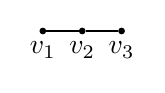
\begin{tikzpicture}[every node/.style={draw, circle, fill=black, minimum size=2pt, inner sep=0pt}]
\node[fill=black, label=below:{$v_{1}$}] (G1N1) at (6,4.5) {};
\node[fill=black, label=below:{$v_{2}$}] (G1N0) at (6.5,4.5) {};
\node[fill=black, label=below:{$v_{3}$}] (G1N2) at (7,4.5) {};
\draw (G1N0) -- (G1N1);
\draw (G1N0) -- (G1N2);
\end{tikzpicture}
\end{document}
};
%        \node[anchor=east] (Lfile1) at (4.5,-2.5) {$(10,9,11)$};
        
%    \end{tikzpicture}
%    \caption{A $\sigma^{+-}$-labeling of $\mathbf{T_{6}^{6}} \sqcup \mathbf{T_{3}^{1}}\sim (4,1,8,5,6,7)\sqcup (10,9,11)$}
%    \label{fig:union_files}
%\end{figure}
    

%%%%%%%%%%%%%%%%%%%%%%%%%%%%%%%%%%%%%%%%%%%%%%%%%%%%%%%%%%%%%%%%%%%%%%%%%%%%%%%%%%%%%%%%%%%%%%%%%
\begin{figure}[H]
    \centering
    \begin{tikzpicture}[scale=0.5]
        %G1

        \node[anchor=east] (file1) at (0, 0) {\documentclass{standalone}
\usepackage{tikz}
\begin{document}
\begin{tikzpicture}[every node/.style={draw, circle, fill=black, minimum size=2pt, inner sep=0pt}]
\node[fill=black, label=above:{$v_{4}$}] (G1N1) at (90:0.5) {};
\node[fill=black, label=above left:{$v_{2}$}] (G1N0) at (90:0) {};
\node[fill=black, label=below right:{$v_{6}$}] (G1N2) at (306:0.5) {};
\node[fill=black, label=below left:{$v_{5}$}] (G1N3) at (234:0.5) {};
\node[fill=black, label=above left:{$v_{1}$}] (G1N4) at (162:0.5) {};
\node[fill=black, label=above right:{$v_{3}$}] (G1N5) at (18:0.5) {};
\draw (G1N0) -- (G1N1);
\draw (G1N0) -- (G1N2);
\draw (G1N0) -- (G1N3);
\draw (G1N0) -- (G1N4);
\draw (G1N0) -- (G1N5);
\end{tikzpicture}
\end{document}
};
        % Union symbol
        
        % Second standalone file
        \node[anchor=west] (file2) at (0.001, -0.62) {\documentclass{standalone}
\usepackage{tikz}
\begin{document}
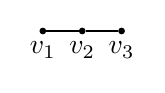
\begin{tikzpicture}[every node/.style={draw, circle, fill=black, minimum size=2pt, inner sep=0pt}]
\node[fill=black, label=below:{$v_{1}$}] (G1N1) at (6,4.5) {};
\node[fill=black, label=below:{$v_{2}$}] (G1N0) at (6.5,4.5) {};
\node[fill=black, label=below:{$v_{3}$}] (G1N2) at (7,4.5) {};
\draw (G1N0) -- (G1N1);
\draw (G1N0) -- (G1N2);
\end{tikzpicture}
\end{document}
};

    \begin{scope}[shift={(3.75,0)}]
        \draw[dashed](0,1.75)--(0,-16.75);
    \end{scope}
%%%%%%%%%%%%%%%%%%%%%%%%%%%%%%%%% second column %%%%%%%%%%%%%%%%%%%%%%%%%%%%%%%%%%%%%%%%%%%%%%%%%

    \begin{scope}[shift = {(7.75,0)}]
        
        \node[anchor=east] (file1) at (0, 0) {\documentclass{standalone}
\usepackage{tikz}
\begin{document}
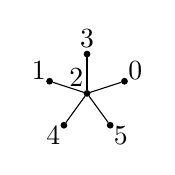
\begin{tikzpicture}[every node/.style={draw, circle, fill=black, minimum size=2pt, inner sep=0pt}]
\node[fill=black, label=above left:{$1$}] (G1N4) at (162:0.5) {};
\node[fill=black, label={[yshift=2pt]above left:{$2$}}] (G1N0) at (90:0) {};
\node[fill=black, label=above right:{$0$}] (G1N5) at (18:0.5) {};
\node[fill=black, label=above:{$3$}] (G1N1) at (90:0.5) {};
\node[fill=black, label=below left:{$4$}] (G1N3) at (234:0.5) {};
\node[fill=black, label=below right:{$5$}] (G1N2) at (306:0.5) {};

\draw (G1N0) -- (G1N1);
\draw (G1N0) -- (G1N2);
\draw (G1N0) -- (G1N3);
\draw (G1N0) -- (G1N4);
\draw (G1N0) -- (G1N5);
\end{tikzpicture}
\end{document}};
        
        \node[anchor=west] (file2) at (0.001, -0.62) {\documentclass{standalone}
\usepackage{tikz}
\begin{document}
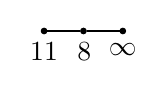
\begin{tikzpicture}[every node/.style={draw, circle, fill=black, minimum size=2pt, inner sep=0pt}]
\node[fill=black, label=below:{$11$}] (G1N1) at (6,4.5) {};
\node[fill=black, label=below:{$\;8\>$}] (G1N0) at (6.5,4.5) {};
\node[fill=black, label=below:{$\infty$}] (G1N2) at (7,4.5) {};
\draw (G1N0) -- (G1N1);
\draw (G1N0) -- (G1N2);
\end{tikzpicture}
\end{document}
};

        \draw[->] (4,0.01) -- (4,0.01) node[draw = none,midway, text=black, fill=white] {$\overset{+7}{\circlearrowright}$};
        %G2
        \node[anchor=east] (file1) at (0, -3) {\documentclass{standalone}
\usepackage{tikz}
\begin{document}
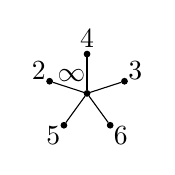
\begin{tikzpicture}[every node/.style={draw, circle, fill=black, minimum size=2pt, inner sep=0pt}]
\node[fill=black, label=above left:{$2$}] (G1N4) at (162:0.5) {};
\node[fill=black, label={[xshift=-0.85,yshift=1.5pt]above left:{$\infty$}}] (G1N0) at (90:0) {};
\node[fill=black, label=above right:{$3$}] (G1N5) at (18:0.5) {};
\node[fill=black, label=above:{$4$}] (G1N1) at (90:0.5) {};
\node[fill=black, label=below left:{$5$}] (G1N3) at (234:0.5) {};
\node[fill=black, label=below right:{$6$}] (G1N2) at (306:0.5) {};

\draw (G1N0) -- (G1N1);
\draw (G1N0) -- (G1N2);
\draw (G1N0) -- (G1N3);
\draw (G1N0) -- (G1N4);
\draw (G1N0) -- (G1N5);
\end{tikzpicture}
\end{document}};
        
        \node[anchor=west] (file2) at (0.001, -3.62) {\documentclass{standalone}
\usepackage{tikz}
\begin{document}
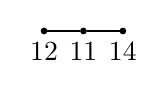
\begin{tikzpicture}[every node/.style={draw, circle, fill=black, minimum size=2pt, inner sep=0pt}]
\node[fill=black, label=below:{$12$}] (G1N1) at (6,4.5) {};
\node[fill=black, label=below:{$11$}] (G1N0) at (6.5,4.5) {};
\node[fill=black, label=below:{$14$}] (G1N2) at (7,4.5) {};
\draw (G1N0) -- (G1N1);
\draw (G1N0) -- (G1N2);
\end{tikzpicture}
\end{document}
};

        \draw[->] (4,-3.01) -- (4,-3.01) node[draw = none,midway, text=black, fill=white] {$\overset{+7}{\circlearrowright}$};
        %G3
        \node[anchor=east] (file1) at (0, -6) {\documentclass{standalone}
\usepackage{tikz}
\begin{document}
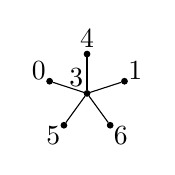
\begin{tikzpicture}[every node/.style={draw, circle, fill=black, minimum size=2pt, inner sep=0pt}]
\node[fill=black, label=above left:{$0$}] (G1N4) at (162:0.5) {};
\node[fill=black, label={[yshift=2pt]above left:{$3$}}] (G1N0) at (90:0) {};
\node[fill=black, label=above right:{$1$}] (G1N5) at (18:0.5) {};
\node[fill=black, label=above:{$4$}] (G1N1) at (90:0.5) {};
\node[fill=black, label=below left:{$5$}] (G1N3) at (234:0.5) {};
\node[fill=black, label=below right:{$6$}] (G1N2) at (306:0.5) {};
\draw (G1N0) -- (G1N1);
\draw (G1N0) -- (G1N2);
\draw (G1N0) -- (G1N3);
\draw (G1N0) -- (G1N4);
\draw (G1N0) -- (G1N5);
\end{tikzpicture}
\end{document}
};
        
        \node[anchor=west] (file2) at (0.001, -6.62) {\documentclass{standalone}
\usepackage{tikz}
\begin{document}
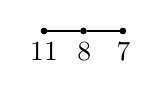
\begin{tikzpicture}[every node/.style={draw, circle, fill=black, minimum size=2pt, inner sep=0pt}]
\node[fill=black, label=below:{$11$}] (G1N1) at (6,4.5) {};
\node[fill=black, label=below:{$\;8\>$}] (G1N0) at (6.5,4.5) {};
\node[fill=black, label=below:{$\;7\>$}] (G1N2) at (7,4.5) {};
\draw (G1N0) -- (G1N1);
\draw (G1N0) -- (G1N2);
\end{tikzpicture}
\end{document}
};

        \draw[->] (4,-6.01) -- (4,-6.01) node[draw = none,midway, text=black, fill=white] {$\overset{+7}{\circlearrowright}$};
        %G4
        \node[anchor=east] (file1) at (0.246, -9) {\documentclass{standalone}
\usepackage{tikz}
\begin{document}
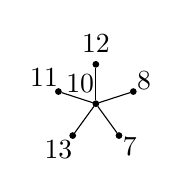
\begin{tikzpicture}[every node/.style={draw, circle, fill=black, minimum size=2pt, inner sep=0pt}]
\node[fill=black, label=above left:{$11$}] (G1N4) at (162:0.5) {};
\node[fill=black, label={[xshift=-0.5,yshift=2pt]above left:{$10$}}] (G1N0) at (90:0) {};
\node[fill=black, label=above right:{$8$}] (G1N5) at (18:0.5) {};
\node[fill=black, label=above:{$12$}] (G1N1) at (90:0.5) {};
\node[fill=black, label=below left:{$13$}] (G1N3) at (234:0.5) {};
\node[fill=black, label=below right:{$7$}] (G1N2) at (306:0.5) {};

\draw (G1N0) -- (G1N1);
\draw (G1N0) -- (G1N2);
\draw (G1N0) -- (G1N3);
\draw (G1N0) -- (G1N4);
\draw (G1N0) -- (G1N5);
\end{tikzpicture}
\end{document}};
        
        \node[anchor=west] (file2) at (0.001, -9.62) {\documentclass{standalone}
\usepackage{tikz}
\begin{document}
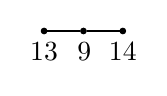
\begin{tikzpicture}[every node/.style={draw, circle, fill=black, minimum size=2pt, inner sep=0pt}]
\node[fill=black, label=below:{$13$}] (G1N1) at (6,4.5) {};
\node[fill=black, label=below:{$\;9\>$}] (G1N0) at (6.5,4.5) {};
\node[fill=black, label=below:{$14$}] (G1N2) at (7,4.5) {};
\draw (G1N0) -- (G1N1);
\draw (G1N0) -- (G1N2);
\end{tikzpicture}
\end{document}
};

        \draw[->] (4,-9.01) -- (4,-9.01) node[draw = none,midway, text=black, fill=white] {$\overset{+1}{\circlearrowright}$};

        %G5
        \node[anchor=east] (file1) at (0.246, -12) {\documentclass{standalone}
\usepackage{tikz}
\begin{document}
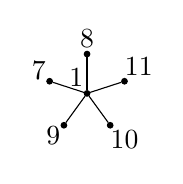
\begin{tikzpicture}[every node/.style={draw, circle, fill=black, minimum size=2pt, inner sep=0pt}]
\node[fill=black, label=above left:{$7$}] (G1N4) at (162:0.5) {};
\node[fill=black, label={[yshift=2pt]above left:{$1$}}] (G1N0) at (90:0) {};
\node[fill=black, label=above right:{$11$}] (G1N5) at (18:0.5) {};
\node[fill=black, label=above:{$8$}] (G1N1) at (90:0.5) {};
\node[fill=black, label=below left:{$9$}] (G1N3) at (234:0.5) {};
\node[fill=black, label=below right:{$10$}] (G1N2) at (306:0.5) {};
\draw (G1N0) -- (G1N1);
\draw (G1N0) -- (G1N2);
\draw (G1N0) -- (G1N3);
\draw (G1N0) -- (G1N4);
\draw (G1N0) -- (G1N5);
\end{tikzpicture}
\end{document}};
        
        \node[anchor=west] (file2) at (0.001, -12.62) {\documentclass{standalone}
\usepackage{tikz}
\begin{document}
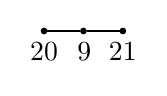
\begin{tikzpicture}[every node/.style={draw, circle, fill=black, minimum size=2pt, inner sep=0pt}]
\node[fill=black, label=below:{$20$}] (G1N1) at (6,4.5) {};
\node[fill=black, label=below:{$\;9\>$}] (G1N0) at (6.5,4.5) {};
\node[fill=black, label=below:{$21$}] (G1N2) at (7,4.5) {};
\draw (G1N0) -- (G1N1);
\draw (G1N0) -- (G1N2);
\end{tikzpicture}
\end{document}};

        \draw[->] (4,-12.01) -- (4,-12.01) node[draw = none,midway, text=black, fill=white] {$\overset{+1}{\circlearrowright}$};
        \end{scope}
        
    \begin{scope}[shift={(12.9555,0)}]
        \draw[dashed](0,1.75)--(0,-16.75);
    \end{scope}
%%%%%%%%%%%%%%%%%%%%%%%%%%%%%%%%% third column %%%%%%%%%%%%%%%%%%%%%%%%%%%%%%%%%%%%%%%%%%%%%%%%%%
    \begin{scope}[shift={(17,0)}]

        %G1
        \node[anchor=east] (file1) at (0, 0) {\documentclass{standalone}
\usepackage{tikz}
\begin{document}
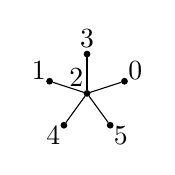
\begin{tikzpicture}[every node/.style={draw, circle, fill=black, minimum size=2pt, inner sep=0pt}]
\node[fill=black, label=above left:{$1$}] (G1N4) at (162:0.5) {};
\node[fill=black, label={[yshift=2pt]above left:{$2$}}] (G1N0) at (90:0) {};
\node[fill=black, label=above right:{$0$}] (G1N5) at (18:0.5) {};
\node[fill=black, label=above:{$3$}] (G1N1) at (90:0.5) {};
\node[fill=black, label=below left:{$4$}] (G1N3) at (234:0.5) {};
\node[fill=black, label=below right:{$5$}] (G1N2) at (306:0.5) {};

\draw (G1N0) -- (G1N1);
\draw (G1N0) -- (G1N2);
\draw (G1N0) -- (G1N3);
\draw (G1N0) -- (G1N4);
\draw (G1N0) -- (G1N5);
\end{tikzpicture}
\end{document}};
        
        \node[anchor=west] (file2) at (0.001, -0.62) {\documentclass{standalone}
\usepackage{tikz}
\begin{document}
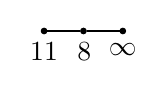
\begin{tikzpicture}[every node/.style={draw, circle, fill=black, minimum size=2pt, inner sep=0pt}]
\node[fill=black, label=below:{$11$}] (G1N1) at (6,4.5) {};
\node[fill=black, label=below:{$\;8\>$}] (G1N0) at (6.5,4.5) {};
\node[fill=black, label=below:{$\infty$}] (G1N2) at (7,4.5) {};
\draw (G1N0) -- (G1N1);
\draw (G1N0) -- (G1N2);
\end{tikzpicture}
\end{document}
};

        \draw[->] (4,0.01) -- (4,0.01) node[draw = none,midway, text=black, fill=white] {$\overset{+7}{\circlearrowright}$};
        %G2
        \node[anchor=east] (file1) at (0, -3) {\documentclass{standalone}
\usepackage{tikz}
\begin{document}
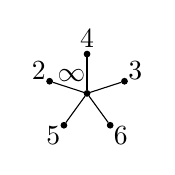
\begin{tikzpicture}[every node/.style={draw, circle, fill=black, minimum size=2pt, inner sep=0pt}]
\node[fill=black, label=above left:{$2$}] (G1N4) at (162:0.5) {};
\node[fill=black, label={[xshift=-0.85,yshift=1.5pt]above left:{$\infty$}}] (G1N0) at (90:0) {};
\node[fill=black, label=above right:{$3$}] (G1N5) at (18:0.5) {};
\node[fill=black, label=above:{$4$}] (G1N1) at (90:0.5) {};
\node[fill=black, label=below left:{$5$}] (G1N3) at (234:0.5) {};
\node[fill=black, label=below right:{$6$}] (G1N2) at (306:0.5) {};

\draw (G1N0) -- (G1N1);
\draw (G1N0) -- (G1N2);
\draw (G1N0) -- (G1N3);
\draw (G1N0) -- (G1N4);
\draw (G1N0) -- (G1N5);
\end{tikzpicture}
\end{document}};
        
        \node[anchor=west] (file2) at (0.001, -3.62) {\documentclass{standalone}
\usepackage{tikz}
\begin{document}
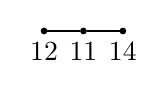
\begin{tikzpicture}[every node/.style={draw, circle, fill=black, minimum size=2pt, inner sep=0pt}]
\node[fill=black, label=below:{$12$}] (G1N1) at (6,4.5) {};
\node[fill=black, label=below:{$11$}] (G1N0) at (6.5,4.5) {};
\node[fill=black, label=below:{$14$}] (G1N2) at (7,4.5) {};
\draw (G1N0) -- (G1N1);
\draw (G1N0) -- (G1N2);
\end{tikzpicture}
\end{document}
};

        \draw[->] (4,-3.01) -- (4,-3.01) node[draw = none,midway, text=black, fill=white] {$\overset{+7}{\circlearrowright}$};
        %G3
        \node[anchor=east] (file1) at (0, -6) {\documentclass{standalone}
\usepackage{tikz}
\begin{document}
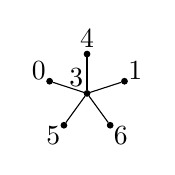
\begin{tikzpicture}[every node/.style={draw, circle, fill=black, minimum size=2pt, inner sep=0pt}]
\node[fill=black, label=above left:{$0$}] (G1N4) at (162:0.5) {};
\node[fill=black, label={[yshift=2pt]above left:{$3$}}] (G1N0) at (90:0) {};
\node[fill=black, label=above right:{$1$}] (G1N5) at (18:0.5) {};
\node[fill=black, label=above:{$4$}] (G1N1) at (90:0.5) {};
\node[fill=black, label=below left:{$5$}] (G1N3) at (234:0.5) {};
\node[fill=black, label=below right:{$6$}] (G1N2) at (306:0.5) {};
\draw (G1N0) -- (G1N1);
\draw (G1N0) -- (G1N2);
\draw (G1N0) -- (G1N3);
\draw (G1N0) -- (G1N4);
\draw (G1N0) -- (G1N5);
\end{tikzpicture}
\end{document}
};
        
        \node[anchor=west] (file2) at (0.001, -6.62) {\documentclass{standalone}
\usepackage{tikz}
\begin{document}
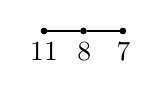
\begin{tikzpicture}[every node/.style={draw, circle, fill=black, minimum size=2pt, inner sep=0pt}]
\node[fill=black, label=below:{$11$}] (G1N1) at (6,4.5) {};
\node[fill=black, label=below:{$\;8\>$}] (G1N0) at (6.5,4.5) {};
\node[fill=black, label=below:{$\;7\>$}] (G1N2) at (7,4.5) {};
\draw (G1N0) -- (G1N1);
\draw (G1N0) -- (G1N2);
\end{tikzpicture}
\end{document}
};

        \draw[->] (4,-6.01) -- (4,-6.01) node[draw = none,midway, text=black, fill=white] {$\overset{+7}{\circlearrowright}$};
        %G4
        \node[anchor=east] (file1) at (0, -9) {\documentclass{standalone}
\usepackage{tikz}
\begin{document}
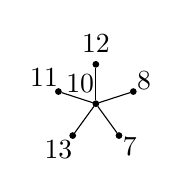
\begin{tikzpicture}[every node/.style={draw, circle, fill=black, minimum size=2pt, inner sep=0pt}]
\node[fill=black, label=above left:{$11$}] (G1N4) at (162:0.5) {};
\node[fill=black, label={[xshift=-0.5,yshift=2pt]above left:{$10$}}] (G1N0) at (90:0) {};
\node[fill=black, label=above right:{$8$}] (G1N5) at (18:0.5) {};
\node[fill=black, label=above:{$12$}] (G1N1) at (90:0.5) {};
\node[fill=black, label=below left:{$13$}] (G1N3) at (234:0.5) {};
\node[fill=black, label=below right:{$7$}] (G1N2) at (306:0.5) {};

\draw (G1N0) -- (G1N1);
\draw (G1N0) -- (G1N2);
\draw (G1N0) -- (G1N3);
\draw (G1N0) -- (G1N4);
\draw (G1N0) -- (G1N5);
\end{tikzpicture}
\end{document}};
        
        \node[anchor=west] (file2) at (0.001, -9.62) {\documentclass{standalone}
\usepackage{tikz}
\begin{document}
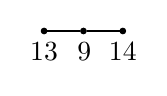
\begin{tikzpicture}[every node/.style={draw, circle, fill=black, minimum size=2pt, inner sep=0pt}]
\node[fill=black, label=below:{$13$}] (G1N1) at (6,4.5) {};
\node[fill=black, label=below:{$\;9\>$}] (G1N0) at (6.5,4.5) {};
\node[fill=black, label=below:{$14$}] (G1N2) at (7,4.5) {};
\draw (G1N0) -- (G1N1);
\draw (G1N0) -- (G1N2);
\end{tikzpicture}
\end{document}
};

        \draw[->] (4,-9.01) -- (4,-9.01) node[draw = none,midway, text=black, fill=white] {$\overset{+7}{\circlearrowright}$};
        
        %G5
        \node[anchor=east] (file1) at (0.246, -12) {\documentclass{standalone}
\usepackage{tikz}
\begin{document}
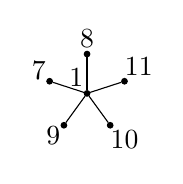
\begin{tikzpicture}[every node/.style={draw, circle, fill=black, minimum size=2pt, inner sep=0pt}]
\node[fill=black, label=above left:{$7$}] (G1N4) at (162:0.5) {};
\node[fill=black, label={[yshift=2pt]above left:{$1$}}] (G1N0) at (90:0) {};
\node[fill=black, label=above right:{$11$}] (G1N5) at (18:0.5) {};
\node[fill=black, label=above:{$8$}] (G1N1) at (90:0.5) {};
\node[fill=black, label=below left:{$9$}] (G1N3) at (234:0.5) {};
\node[fill=black, label=below right:{$10$}] (G1N2) at (306:0.5) {};
\draw (G1N0) -- (G1N1);
\draw (G1N0) -- (G1N2);
\draw (G1N0) -- (G1N3);
\draw (G1N0) -- (G1N4);
\draw (G1N0) -- (G1N5);
\end{tikzpicture}
\end{document}};
        
        \node[anchor=west] (file2) at (0.001, -12.62) {\documentclass{standalone}
\usepackage{tikz}
\begin{document}
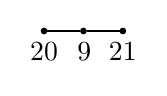
\begin{tikzpicture}[every node/.style={draw, circle, fill=black, minimum size=2pt, inner sep=0pt}]
\node[fill=black, label=below:{$20$}] (G1N1) at (6,4.5) {};
\node[fill=black, label=below:{$\;9\>$}] (G1N0) at (6.5,4.5) {};
\node[fill=black, label=below:{$21$}] (G1N2) at (7,4.5) {};
\draw (G1N0) -- (G1N1);
\draw (G1N0) -- (G1N2);
\end{tikzpicture}
\end{document}};

        \draw[->] (4,-12.01) -- (4,-12.01) node[draw = none,midway, text=black, fill=white] {$\overset{+1}{\circlearrowright}$};

        %G6
        \node[anchor=east] (file1) at (0.246, -15) {\documentclass{standalone}
\usepackage{tikz}
\begin{document}
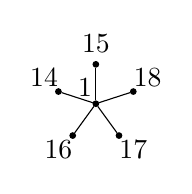
\begin{tikzpicture}[every node/.style={draw, circle, fill=black, minimum size=2pt, inner sep=0pt}]
\node[fill=black, label=above left:{$14$}] (G1N4) at (162:0.5) {};
\node[fill=black, label={[yshift=2pt]above left:{$1$}}] (G1N0) at (90:0) {};
\node[fill=black, label=above right:{$18$}] (G1N5) at (18:0.5) {};
\node[fill=black, label=above:{$15$}] (G1N1) at (90:0.5) {};
\node[fill=black, label=below left:{$16$}] (G1N3) at (234:0.5) {};
\node[fill=black, label=below right:{$17$}] (G1N2) at (306:0.5) {};
\draw (G1N0) -- (G1N1);
\draw (G1N0) -- (G1N2);
\draw (G1N0) -- (G1N3);
\draw (G1N0) -- (G1N4);
\draw (G1N0) -- (G1N5);
\end{tikzpicture}
\end{document}
};
        
        \node[anchor=west] (file2) at (0.001, -15.62) {\documentclass{standalone}
\usepackage{tikz}
\begin{document}
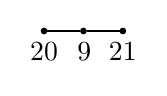
\begin{tikzpicture}[every node/.style={draw, circle, fill=black, minimum size=2pt, inner sep=0pt}]
\node[fill=black, label=below:{$20$}] (G1N1) at (6,4.5) {};
\node[fill=black, label=below:{$\;9\>$}] (G1N0) at (6.5,4.5) {};
\node[fill=black, label=below:{$21$}] (G1N2) at (7,4.5) {};
\draw (G1N0) -- (G1N1);
\draw (G1N0) -- (G1N2);
\end{tikzpicture}
\end{document}};

        \draw[->] (4,-15.01) -- (4,-15.01) node[draw = none,midway, text=black, fill=white] {$\overset{+1}{\circlearrowright}$};

    \end{scope}
    \end{tikzpicture}
    \caption{A $\sigma^{+-}$-labeling of $F \cong\mathbf{T_{6}^{6}} \sqcup \mathbf{T_{3}^{1}}$ (left) and generating presentations for the $F$-decomposition of $K_{n}$ where $n=35$ (middle) and $n=36$ (right)}
    \label{fig:7mod14example}
\end{figure}